\documentclass[12pt,openright,oneside,a4paper,brazil]{abntex2}
\usepackage[utf8]{inputenc}
\counterwithout{section}{section}
\counterwithout{figure}{chapter}
\counterwithout{table}{chapter}
\setlength{\parindent}{1.3cm}
\usepackage{indentfirst}
\setlength{\parskip}{0.2cm}
\usepackage[bottom=2cm,top=3cm,left=3cm,right=2cm]{geometry}
\usepackage{graphicx}
\graphicspath{{figuras/}}
\usepackage{placeins}

%opening
\title{}
\author{}

\begin{document}
\textual
\begin{center}
 {\large Plano de gerenciamento de Tempo}\\[0.2cm]
 {Planta de abastecimento de água potável a partir da umidade do ar}\\
 \end{center}
 
 \section{Histórico de Alterações}
\begin{table}[h]
\centering
\begin{tabular}{|c|c|p{6cm}|p{5cm}|}

Data & Versão & Descrição & Responsável\\
\hline                               
22/04/2015 & 0.0 & Criação do plano de gerenciamento de escopo & Rafael Abreu de Carvalho, Filippe Leal, Ítalo Paiva Batista. \\
\hline
\end{tabular}
\end{table}

\section{Objetivo}
O objetivo desse plano é estabelecer um processo de gerenciamento do escopo do projeto.

\section{Descrição dos processos de gerenciamento de escopo}
O escopo produzido para a realização do projeto foi baseado em um documento padrão do projeto proposto, no qual era apresentados a ideia principal e os requisitos que o produto final do projeto deveria suprir ao final do processo, também foi feita uma pesquisa completa sobre as características região escolhida, sobre as características da população residente no local e sobre as tecnologias disponíveis no mercado, o qual suprirá os requisitos apresentados anteriormente. Durante a elaboração do escopo foram criadas uma EAP (estrutura analítica de processo) e uma análise de riscos por meio de uma estrutura Fishbone, documentos primordiais para a decisão do escopo em questão.

As regras para mudanças de escopo foram definidas em cima de características que visam respeitar o espaço determinado no inicio, respeitar os requisito determinados pela proposta inicial do projeto, respeitar as características do local, respeitar a ideia de custo e eficiência e respeitar as necessidades da população local. Tais mudanças deverão ser embasadas por pesquisa cientificas concreta e com alerta prévio.

\section{Priorização das mudanças do escopo e respostas}
As mudanças serão priorizadas para suprir as alterações e consequências que refletiram no quesito de requisitos primordiais do projeto, depois dessa analise os outros quesitos de mudança serão analisados e efetivados no escopo.

\section{Gerenciamento das Configurações (GC)}
\begin{figure}[!ht]
\centering
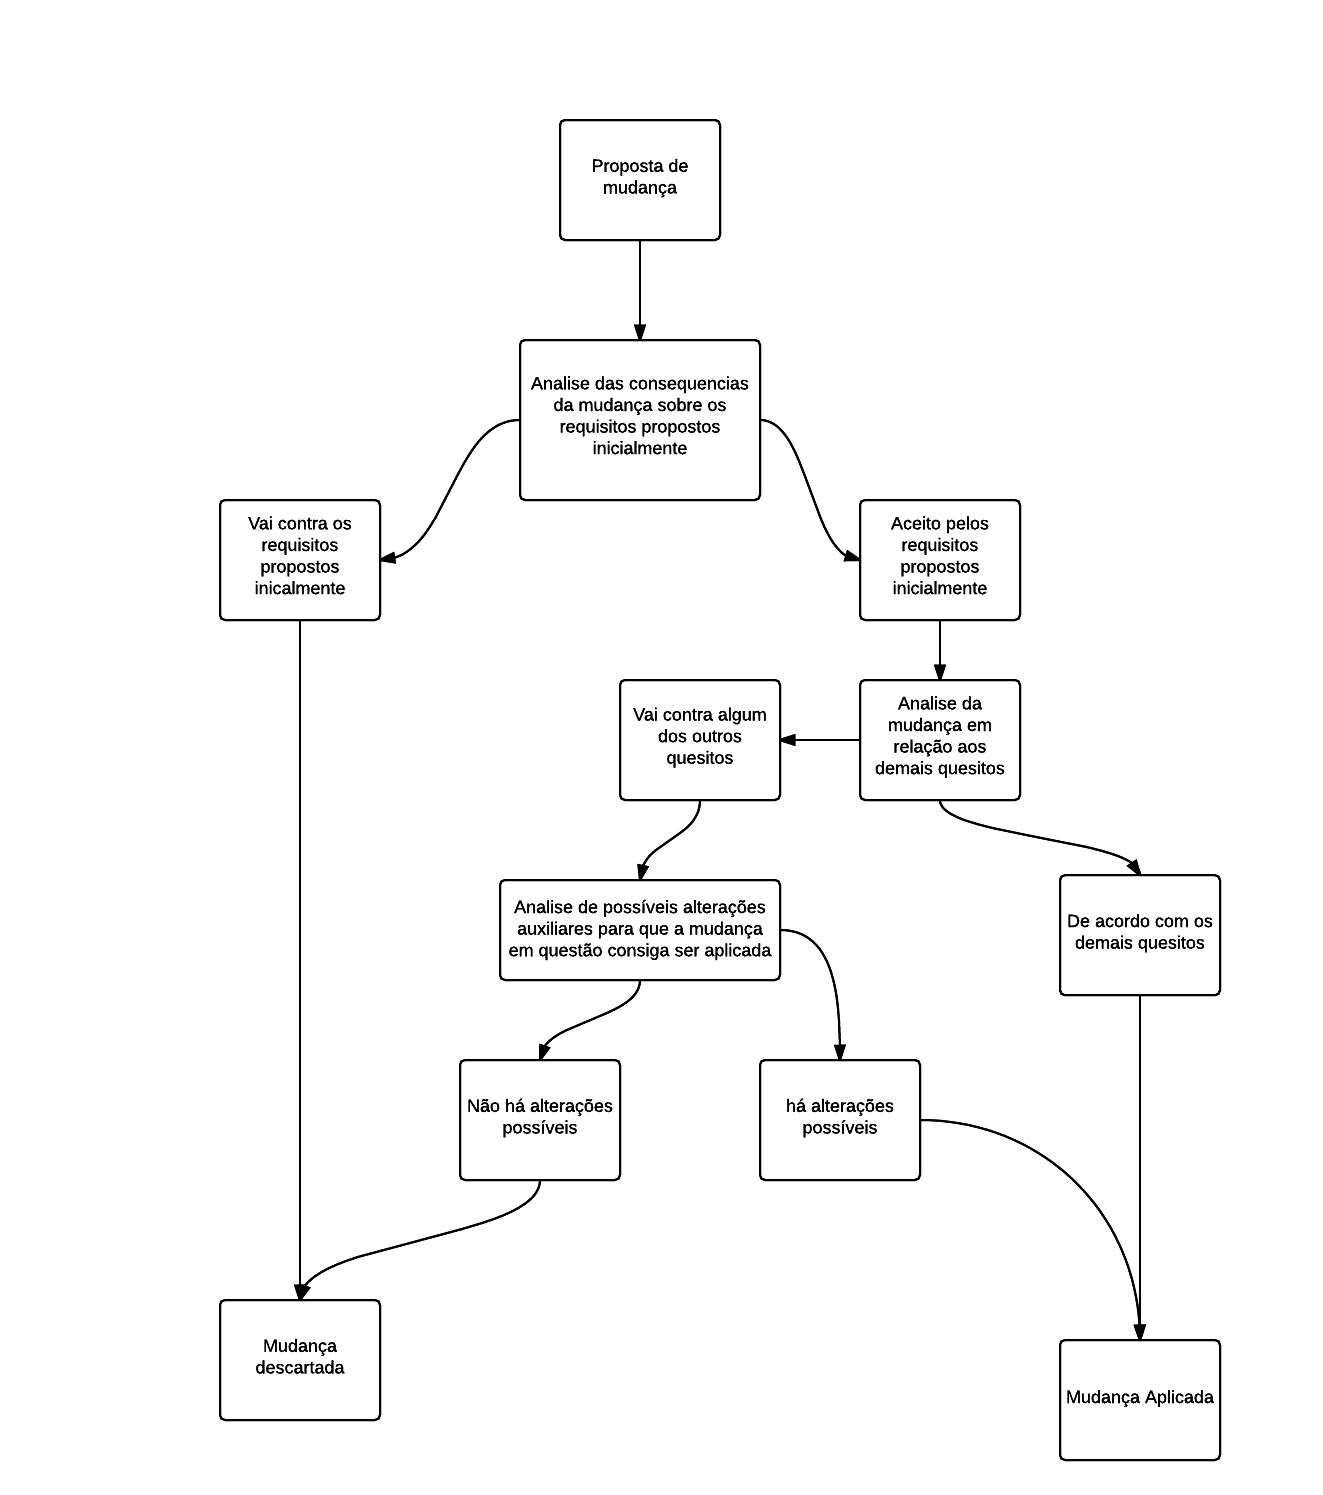
\includegraphics[scale=0.5]{configuracoes}
\label{Rotulo}
\end{figure}
\FloatBarrier

\section{Frequência de avaliação do escopo do projeto.}
O escopo final não sofreu grandes mudanças, devido a fato do mesmo ter surgido após muitas pesquisas e reuniões de grupo, então a frequência de mudanças foi praticamente nula.

\section{Alocação financeira das mudanças de escopo.}
Não houve mudanças impactantes na área de custos do projeto depois da finalização do escopo. Caso houve tais mudanças as mesmas seriam feita de forma a balancear o custo de uma área com os das outras áreas priorizando a parte de tecnologia necessária para que o projeto funcione.

\section{Administração do plano de gerenciamento de escopo:}
\begin{enumerate}

\item Responsável pelo plano:
\begin{itemize}
\item Rafael Abreu de Carvalho
\item Ítalo Paiva Batista

\end{itemize}

\item Freqüência de atualização do plano de gerenciamento de escopo
Como não houve mudanças no escopo depois de definido o documento final, a frequência de atualização foi nula.
\end{enumerate}

\section{Outros assuntos relacionados ao gerenciamento do escopo do projeto não previstos nesse plano}
A única mudança feita foi uma revisão para deixa-lo mais claro e objetivo para o escopo ficar melhor de ser entendido

\section{Assinaturas}
\begin{center}
Data: \rule{0.5cm}{0.1mm}/\rule{0.5cm}{0.1mm}/\rule{1cm}{0.1mm}     \\
\rule{13cm}{0.1mm}\\
ADRIANNY VIANA DE ARAÚJO AMORIM – GERENTE DE PROJETO\\
\rule{13cm}{0.1mm}\\
ÍTALO PAIVA BATISTA - GERENTE DE TEMPO

\end{center}
\end{document}